\section{Finite Automata and Regular Expressions}

The main result of the last section was that the class of languages accepted by finite automata remains the same even if a new and seemingly powerful feature -\textit{nondeterminism}- is allowed. This suggests that the class of languages accepted by finite automata has a sort of \textit{stability}: Two different approaches, one apparently more powerful than the other, end up defining the same class. In this section we shall prove another important characterization of this class of languages, further evidence of how remarkably stable it is: The class of languages accepted by finite automata, deterministic or nondeterministic, is the same as the class of \textit{regular languages} -those that can be described by regular expressions.

\begin{theorem}{}
  The class of languages accepted by finite automata is closed under 
  \begin{enumerate}[label=\alph*)]
    \item union
    \item concatenation
    \item Kleene star
    \item complementation
    \item intersection
  \end{enumerate}
\end{theorem}

\begin{proof}
  In each case we show how to construct an automaton $M$ that accepts the appropriate language, given two automata $M_1$ and $M_2$ (only $M_1$ in the cases of Kleene star and complementation).

  \begin{enumerate}[label=(\alph*)]
    % (a) Union
    \item \textit{Union.}
    Let $M_1 = (K_1, \Sigma, \Delta_1, s_1, F_1)$ and $M_2 = (K_2, \Sigma, \Delta_2, s_2, F_2)$ be nondeterministic finite automata; we shall construct a nondeterministic finite automaton $M$ such that $L(M) = L(M_1) \cup L(M_2)$. The construction of $M$ is rather simple and intuitively clear, illustrated in Figure 8. Basically, $M$ uses nondeterminism to guess whether the input is in $L(M_1)$ or in $L(M_2)$, and then processes the string exactly as the corresponding automaton would; it follows that $L(M) = L(M_1) \cup L(M_2)$. But let us give the formal details and proof for this case.
    \begin{figure}[h!]
      \centering
      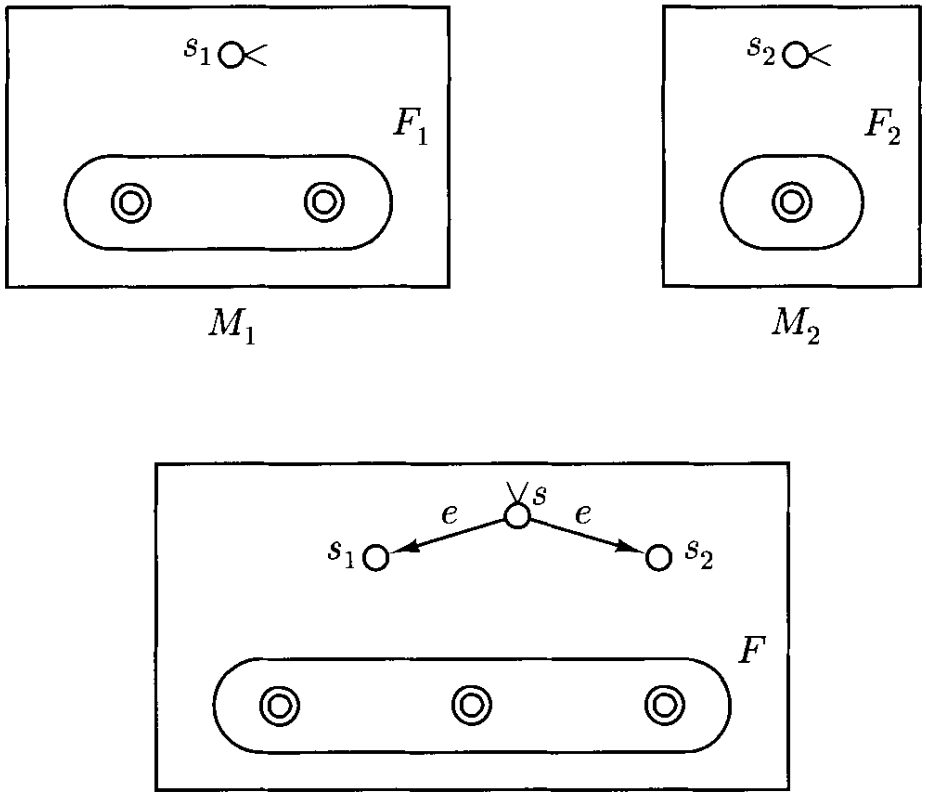
\includegraphics[width=.5\textwidth]{img/Fig2.11.png}
      \caption{}
    \end{figure}
    Without loss of generality, we may assume that $K_1$ and $K_2$ are disjoint sets. Then the finite automaton $M$ that accepts $L(M_1) \cup L(M_2)$ is defined as follows
    
    \quad $M = (K, \Sigma, \Delta, s, F)$, where $s$ is a new state not in $K_1$ or $K_2$,
    \begin{itemize}
      \item $K = K_1 \cup K_2 \cup \left\{ s \right\}$
      \item $F = F_1 \cup F_2$
      \item $\Delta = \Delta_1 \cup \Delta_2 \cup \left\{ (s,e,s_1),(s,e,s_2) \right\}$
    \end{itemize}
    That is, $M$ begins any computation by nondeterministically choosing to enter either the initial state of $M_1$ or the initial state of $M_2$ ,and thereafter, $M$ imitates either $M_1$ or $M_2$. Formally, if $w \in \Sigma^*$, then $(s, w) \vdash^*_M (q, e)$ for some $q \in F$ if and only if either $(s_1, w) \vdash^*_{M_1} (q, e)$ for some $q \in F_2$, or $(s_2, w) \vdash^*_{M_2} (q, e)$ for some $q \in F_2$. Hence $M$ accepts $w$ if and only if $M_1$ accepts $w$ or $M_2$ accepts $w$, and $L(M) = L(M_1) \cup L(M_2)$.

    % (b) Concatenation
    \item \textit{Concatenation.}
    Again, let $M_1$ and $M_2$ be nondeterministic finite automata; we construct a nondeterministic finite automaton $M$ such that $L(M) = L(M_1) L(M_2)$. The construction is shown schematically in Figure 9; $M$ now operates by simulating $M_1$ for a while, and then ``\textit{jumping}'' nondeterministically from a final state of $M_1$ to the initial state of $M_2$. Thereafter, $M$ imitates $M_2$. 

    \begin{figure}[h!]
      \centering
      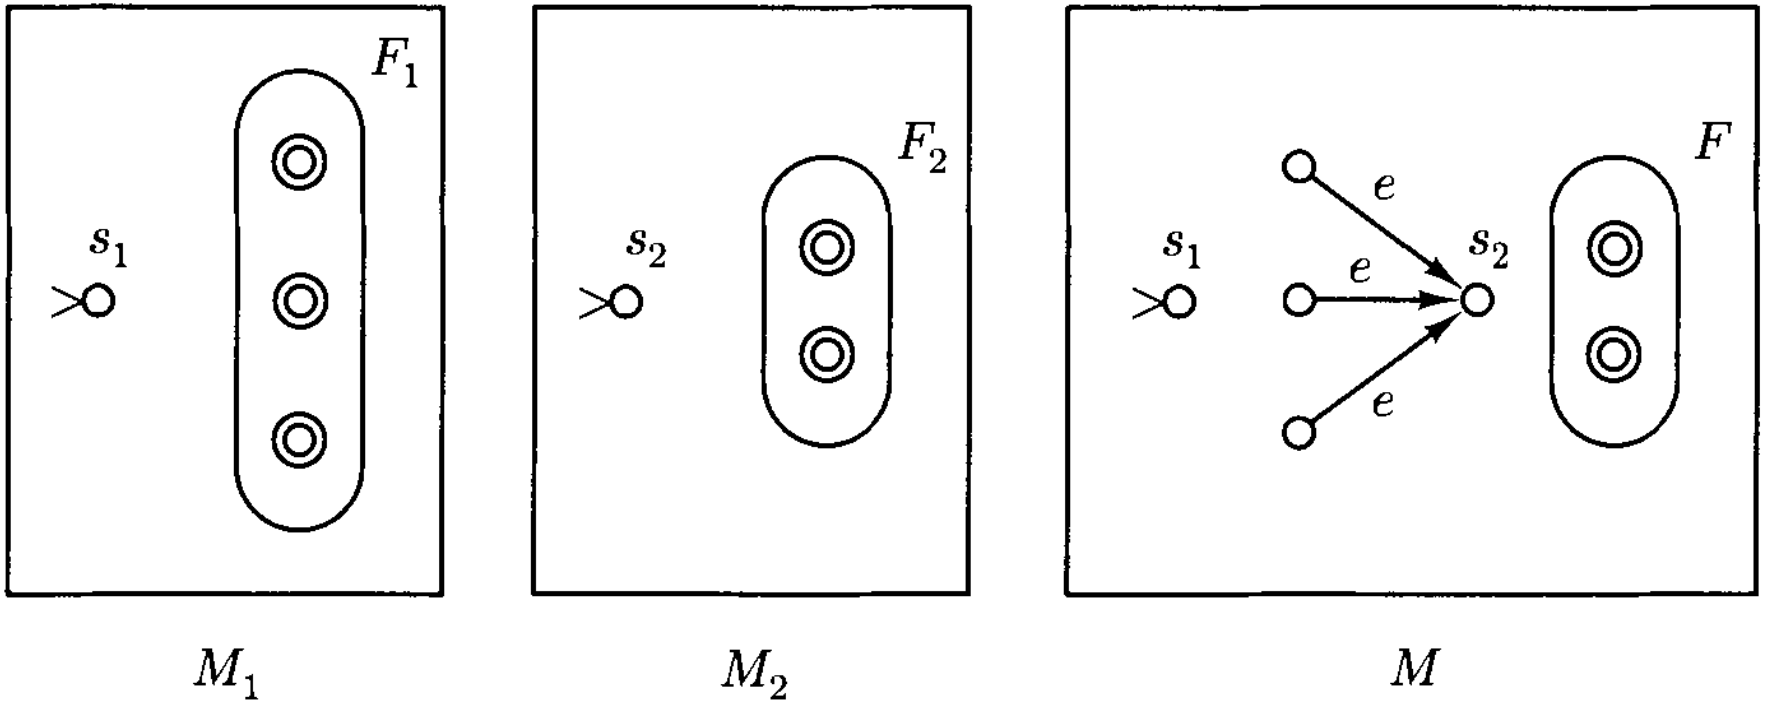
\includegraphics[width=.5\textwidth]{img/Fig2.12.png}
      \caption{}
    \end{figure}

    Then the finite automaton $M$ that accepts $L(M_1) L(M_2)$ is defined as follows (\textit{May include mistakes})
    
    \quad $M = (K, \Sigma, \Delta, s, F)$
    \begin{itemize}
      \item $s = s_1$
      \item $K = K_1 \cup K_2$
      \item $F = F_2$
      \item $\Delta = \Delta_1 \cup \Delta_2 \cup \left\{ (f,e,s_2)\ |\ f \in F_1 \right\}$
    \end{itemize}

    % (c) Kleenestar
    \item \textit{Kleene star.}
    Let $M_1$ be a nondeterministic finite automaton; we construct a nondeterministic finite automaton $M$ such that $L(M) = L(M_1)^*$. The construction is similar to that for concatenation, and is illustrated in Figure 10. $M$ consists of the states of $M_1$ and all the transitions of $M_1$; any final state of $M_1$ is a final state of $M$. In addition, $M$ has a new initial state $s$. This new initial state is also final, so that $e$ is accepted. From $s$ there is an $e$-transition to the initial state $s_1$ of $M_1$, so that the operation of $M_1$ can be initiated after $M$ has been started in state $s$. Finally, $e$-transitions are added from each final state of $M_1$ back to $s_1$; this way, once a string in $L(M_1)$ has been read, computation can resume from the initial state of $M_1$.

    \begin{figure}[h!]
      \centering
      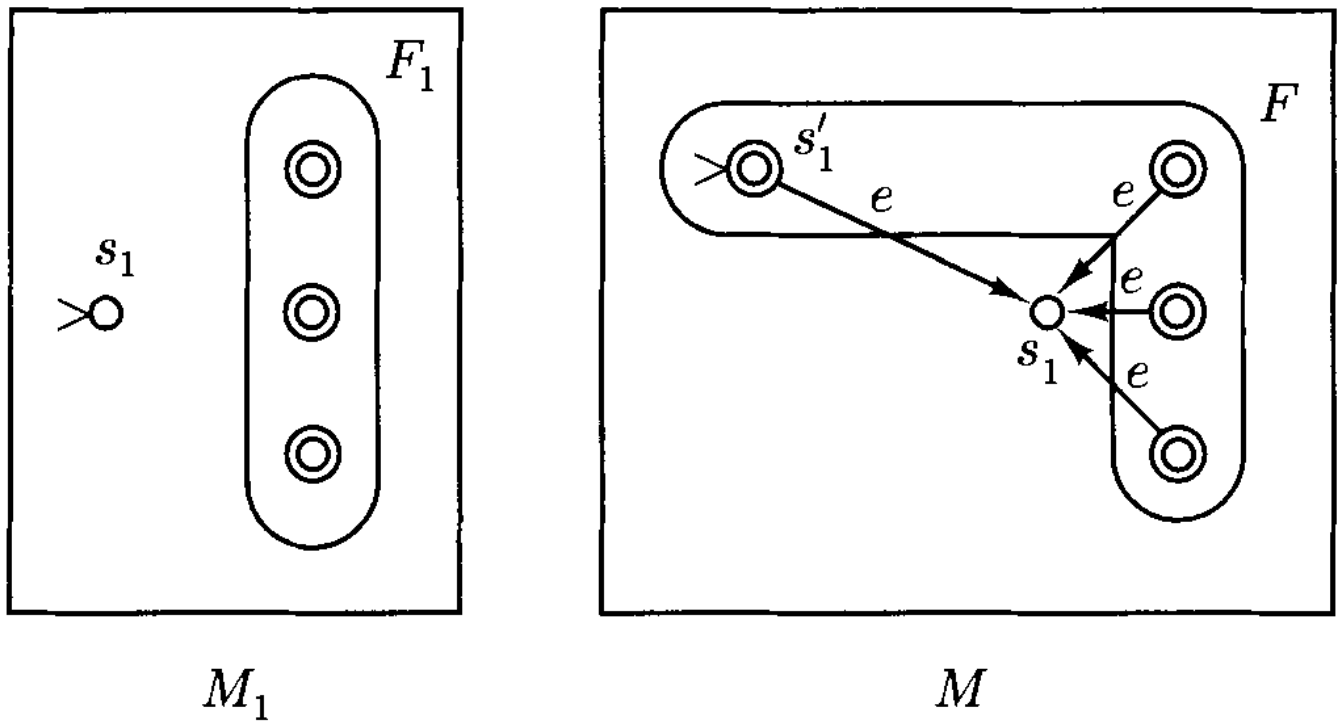
\includegraphics[width=.40\textwidth]{img/Fig2.13.png}
      \caption{}
    \end{figure}

    Then the finite automaton $M$ that accepts $L(M_1)^*$ is defined as follows (\textit{May include mistakes})

    \quad $M = (K, \Sigma, \Delta, s, F)$, where $s$ is not in $M_1$
    \begin{itemize}
      \item $K = K_1 \cup \left\{ s \right\}$
      \item $F = F_1 \cup \left\{ s \right\}$
      \item $\Delta = \Delta_1 \cup \left\{ (s,e,s_1) \right\}$
    \end{itemize}

    % (d) Complementation
    \item \textit{Complementation.}
    Let $M = (K, \Sigma, \delta, s, F)$ be a \textit{deterministic} finite automaton. Then the complementary language $\overline{L} = \Sigma^* - L(M)$ is accepted by the deterministic finite automaton $M = (K, \Sigma, \delta, s, K - F)$. That is, $\overline{M}$ is identical to $M$ except that final and non final states are interchanged.

    Then the finite automaton $M$ that accepts $\overline{L(M_1)}$ is defined as follows (\textit{May include mistakes})

    \quad $M = (K, \Sigma, \Delta, s, F)$.
    \begin{itemize}
      \item $s = s_1$
      \item $K = K_1$
      \item $F = K \setminus F_1$
      \item $\Delta = \Delta_1$
    \end{itemize}

    % (e) Intersection
    \item \textit{Intersection.}
    Just recall that
    \begin{equation*}
      L_1 \cap L_2 = \Sigma^* - \left( \left( \Sigma^* - L_1 \right) \cup \left( \Sigma^* - L_2 \right) \right)
    \end{equation*}
    and so closedness under intersection follows from closedness under union and complementation ((a) and (d) above). So, basically
    \begin{equation*}
      L(M) = L(M_1) \cap L(M_2) = \overline{\overline{L(M_1)} \cup \overline{L(M_2)}}
    \end{equation*}
  \end{enumerate}
\end{proof}

\begin{theorem}{}
  \textit{A language is regular if and only if it is accepted by a finite automaton.}
\end{theorem}

\begin{proof}
  \begin{itemize}
    \item \textit{Only if}. Recall that the class of regular languages is the smallest class of languages containing the empty set $\emptyset$ and the singletons $a$, where $a$ is a symbol, and \textit{closed under union, concatenation, and Kleene star}.

    It is evident (see Figure 11) that the empty set and all singletons are indeed accepted by finite automata; and by Theorem 2 the finite automaton languages are closed under \textit{union}, \textit{concatenation}, and \textit{Kleene star}. Hence \textit{every regular language is accepted by some finite automaton}.

    \begin{example}{}
      Consider the regular expression $(ab \cup aab)^*$. A nondeterministic finite automaton accepting the language denoted by this regular expression can be built up using the methods in the proof of the various parts of Theorem 2, as illustrated in Figure 11.
    \end{example}

    \begin{figure}[h!]
      \centering
      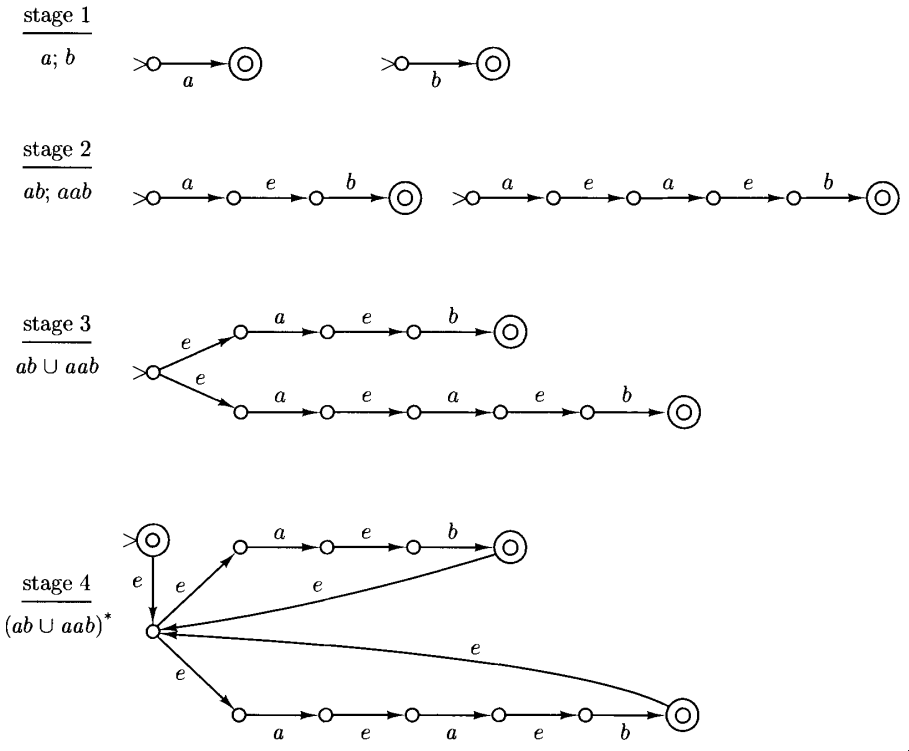
\includegraphics[width=.95\textwidth]{img/Fig2.14.png}
      \caption{}
    \end{figure}

    
    \item \textit{If}. Let $M = (K, \Sigma, \Delta, s, F)$ be a finite automaton (not necessarily deterministic). We shall construct a regular expression $R$ such that $L(R) = L(M)$. We shall represent $L(M)$ as the union of many (but a finite number of) simple languages. Let $K = \left\{ q_1, ..., q_n  \right\}$ and $s = q_1$. For $i, j = 1, ..., n$ and $k = 0, ..., n$:
    \begin{quote}
      $R(i, j, k)$: the set of strings $w \in \Sigma^*$ that can be read by $M$ starting from $q_i$ to $q_j$ without passing through an intermediate state from $\left\{ q_{k+1}, ..., q_n \right\}$ -the endpoints $q_i$ and $q_j$ are allowed to be numbered higher than $k$.
    \end{quote}
    That is, $R(i, j, k)$ is the set of strings spelled by all paths from $q_i$ to $q_j$ of rank $k$ (recall the similar maneuver in the computation of the reflexive-transitive closure of a relation, in which we again considered paths with progressively higher and higher-numbered intermediate nodes). When $k = n$, it follows that
    \begin{equation*}
      R(i,j,n) = \left\{ w \in \Sigma^*\ |\ (q_i, w) \vdash^*_M (q_j, e) \right\}
    \end{equation*}
    Therefore,
    \begin{equation*}
      L(M) = \bigcup \left\{ R(1, j, n)\ |\ q_j \in F \right\}
    \end{equation*}
    The crucial point is that all of these sets $R(i, j, k)$ are regular, and hence so is $L(M)$.

    \quad The proof that each $R(i, j, k)$ is regular is by induction on $k$. For $k = 0$, $R(i, j, 0)$:
    \begin{itemize}
      \item $\left\{ a \in \Sigma \cup \left\{ e \right\}\ |\ (q_i, a, q_j) \in \Delta \right\}$ if $i\neq j$
      \item $\left\{ e \right\} \cup \left\{ a \in \Sigma \cup \left\{ e \right\}\ |\ (q_i, a, q_j) \in \Delta \right\}$ if $i = j$.
    \end{itemize}
    $R(i, j, 0)$ is either singleton or empty for each $i$, $j$, hence regular.

    \quad For the induction step, suppose that $R(i, j, k-1)$ for all $i$, $j$ have been defined as regular languages for all $i$, $j$. Then each set $R(i, j, k)$ can be defined combining previously defined regular languages by the regular operations of union, Kleene star, and concatenation, as follows:
    \begin{equation*}
      R(i, j, k) = R(i, j, k - 1) \cup R(i, k, k - 1) R(k, k, k - 1)^* R(k, j, k - 1)
    \end{equation*}
    This equation states that to get from $q_i$ to $q_j$ without passing through a state numbered greater than $k$, $M$ may either
    \begin{enumerate}
      \item go from $q_i$ to $q_j$ without passing through a state numbered greater than $k - 1$; or
      \item go (a) from $q_i$ to $q_k$; then (b) from $q_k$ to $q_k$ zero or more times; then (c) from $q_k$ to $q_j$; in each case without passing through any intermediate states numbered greater than $k - 1$
    \end{enumerate}
    Consequently, if $R(i, j, k - 1)$ is regular for each $i$, $j$, then $R(i, j, k)$ is also regular for all $i$, $j$, $k$. By induction, $R(i, j, n)$ is regular.
  \end{itemize}
\end{proof}

The proof of the theorem is used to generate a regular expression from a finite state automaton. Its application is simpler when the automaton is in the following special form
\begin{itemize}
  \item the automaton has a single final state, $F = \{f\}$
  \item the initial state does not have an incoming transition
  \item the final state does not have an outgoing transition
\end{itemize}

\noindent Every automaton can be converted to an equivalent automaton in special form.

\quad RE construction from FA:
\begin{enumerate}
  \item Convert FA to an NFA in special form.
  \item For each $k = 0, ..., n$, and for each $i, j = 1, ..., n$: Compute $R(i, j, k)$
  \item Return $R(s, f, n)$
\end{enumerate}


\begin{figure}[t]
  \centering
  \begin{minipage}{.35\textwidth}
    \centering
    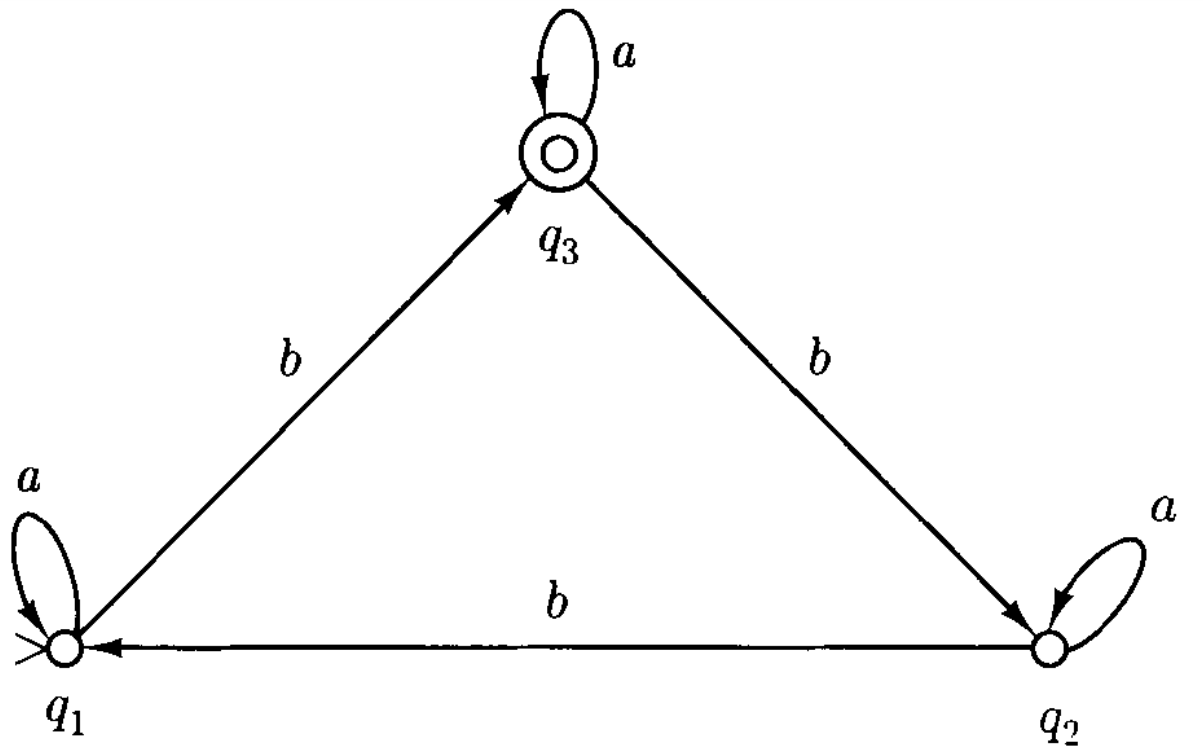
\includegraphics[width=\textwidth]{img/Fig2.15.png}
    \caption{}
  \end{minipage}
  \begin{minipage}{.43\textwidth}
    \centering
    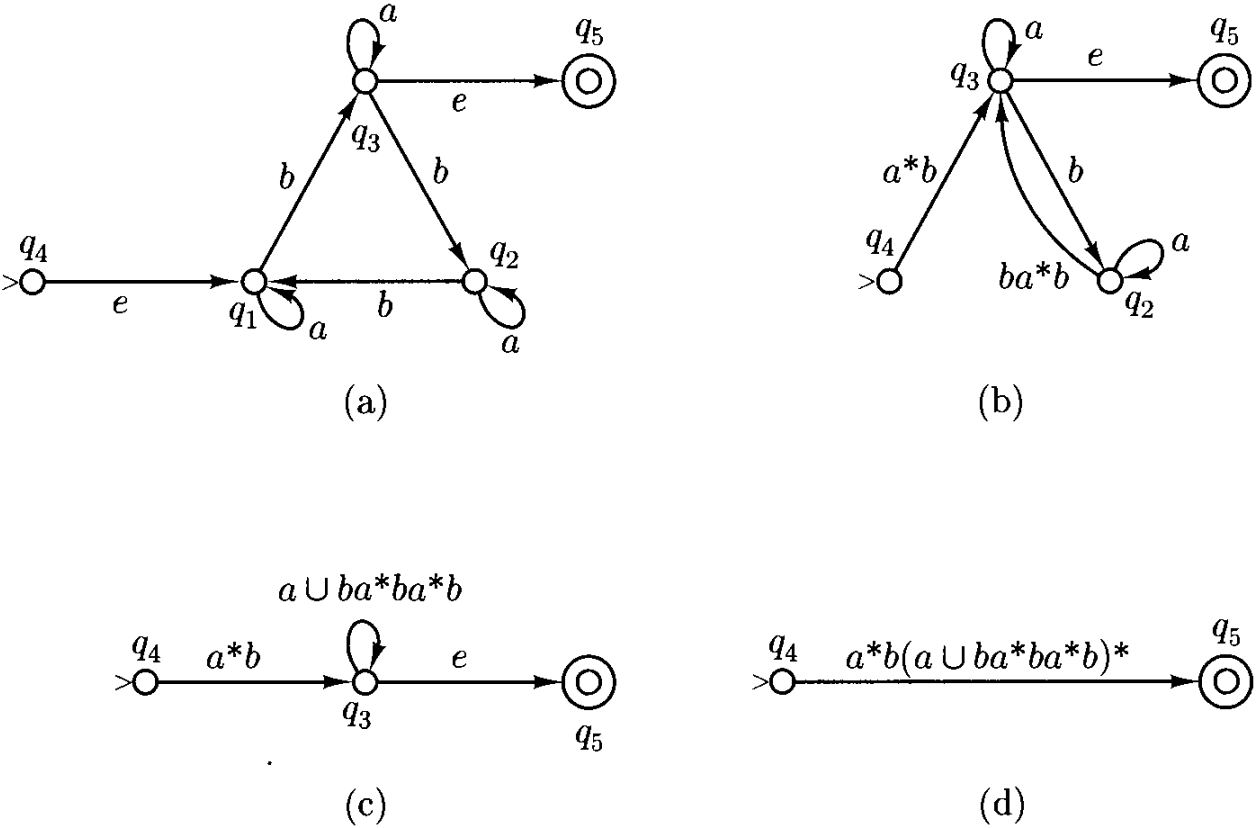
\includegraphics[width=\textwidth]{img/Fig2.16.png}
    \caption{}
  \end{minipage}
\end{figure}

\begin{examplebreak}{}
  Let us construct a regular expression for the language accepted by the deterministic finite automaton of Figure 12. This automaton accepts the language
  \begin{equation*}
    \left\{ w \in \left\{ a, b \right\}^*\ |\ w \textnormal{ has } 3k+1\ b\textnormal{'s for some } k \in \mathbb{N} \right\}\
  \end{equation*}
  Carrying out explicitly the construction of the proof of the \textit{if} part can be very tedious (in this simple case, thirty-six regular expressions would have to be constructed!).
  
  Things are simplified considerably if we assume that the nondeterministic automaton $M$ has two simple properties:
  \begin{itemize}
    \item It has a single final state, $F = \left\{ f \right\}$
    \item Furthermore, if $(q, u, p) \in \Delta$, then $q \neq f$ and $p \neq s$; that is, there are no transitions into the initial state, nor out of the final state
  \end{itemize}
  This ``special form'' is not a loss of generality, because we can add to any automaton $M$ a new initial state $s$ and a new final state $f$, together with $e$-transitions from $s$ to the initial state of $M$ and from all final states of $M$ to $f$ (see Figure 13(a), where the automaton of Figure 12 is brought into this ``special form''). Number now the states of the automaton $q_1, q_2, ..., q_n$, as required by the construction, so that $s = q_{n-1}$ and $f = q_n$. Obviously, the regular expression sought is $R(n - 1, n, n)$.

  \quad We shall compute first the $R(i, j, 0)$'s, from them the $R(i, j, 1)$'s, and so on, as suggested by the proof. At each stage we depict each $R(i, j, k)$'s as a label on an arrow going from state $q_i$ to state $q_j$. We omit arrows labeled by $\emptyset$, and self-loops labeled $\{e\}$. With this convention, the initial automaton depicts the correct values of the $R(i, j, 0)$'s -see Figure 13(a). (This is so because in our initial automaton it so happens that, for each pair of states $(q_i, q_j)$ there is at most one transition of the form $(q_i, u, q_j)$ in $\Delta$. In another automaton we might have to combine by union all transitions from $q_i$ to $q_j$, as suggested by the proof.)

  \quad Now we compute the $R(i, j, 1)$'s; they are shown in Figure 13(b). Notice immediately that state $q_1$ need not be considered in the rest of the construction; all strings that lead $M$ to acceptance passing through state $q_1$ have been considered and taken into account in the $R(i, j, 1)$'s. We can say that state $q_1$ has been \textit{eliminated}. In some sense, we have transformed the finite automaton of Figure 13(a) to an equivalent \textit{generalized finite automaton}, with transitions that may be labeled not only by symbols in $\Sigma$ or $e$, but by entire \textit{regular expressions}. The resulting generalized finite automaton has one less state than the original one, since $q_1$ has been eliminated.

  \quad Let us examine carefully what is involved in general in eliminating a state $q$ (see Figure 14). For each pair of states $q_i \neq q$ and $q_j \neq q$, such that there is an arrow labeled $\alpha$: from $q_i$ to $q$ and an arrow labeled $\beta$ from $q$ to $q_j$, we add an arrow from $q_i$ to $q_j$ labeled $\alpha \gamma^0 \beta$, where $\gamma$ is the label of the arrow from $q$ to itself (if there is no such arrow, then $\gamma = \emptyset$, and thus $\gamma^* = \{e\}$, so the label becomes $\alpha \beta$. If there was already an arrow from $q_i$ to $q_j$ labeled $\delta$, then the new arrow is labeled $\delta \cup \alpha \gamma^* \beta$.

  \quad Continuing like this, we eliminate state $q_2$ to obtain the $R(i, j, 2)$'s in Figure 13(c), and finally we eliminate $q_3$. We have now deleted all states except the initial and final ones, and the generalized automaton has been reduced to a single transition from the initial state to the final state. We can now read the regular expression for $M$ as the label of this transition:
  \begin{equation*}
    R = R(4, 5, 5) = R(4, 5, 3) = a^* b (b a^* b a^* b \cup a)^*
  \end{equation*}
  which is indeed $\left\{ w \in \{a,b\}^*\ |\ w \textnormal{ has } 3k + 1\ b\textnormal{'s for some } k \in \mathbb{N}  \right\}$.
\end{examplebreak}

\begin{figure}[b]
  \centering
  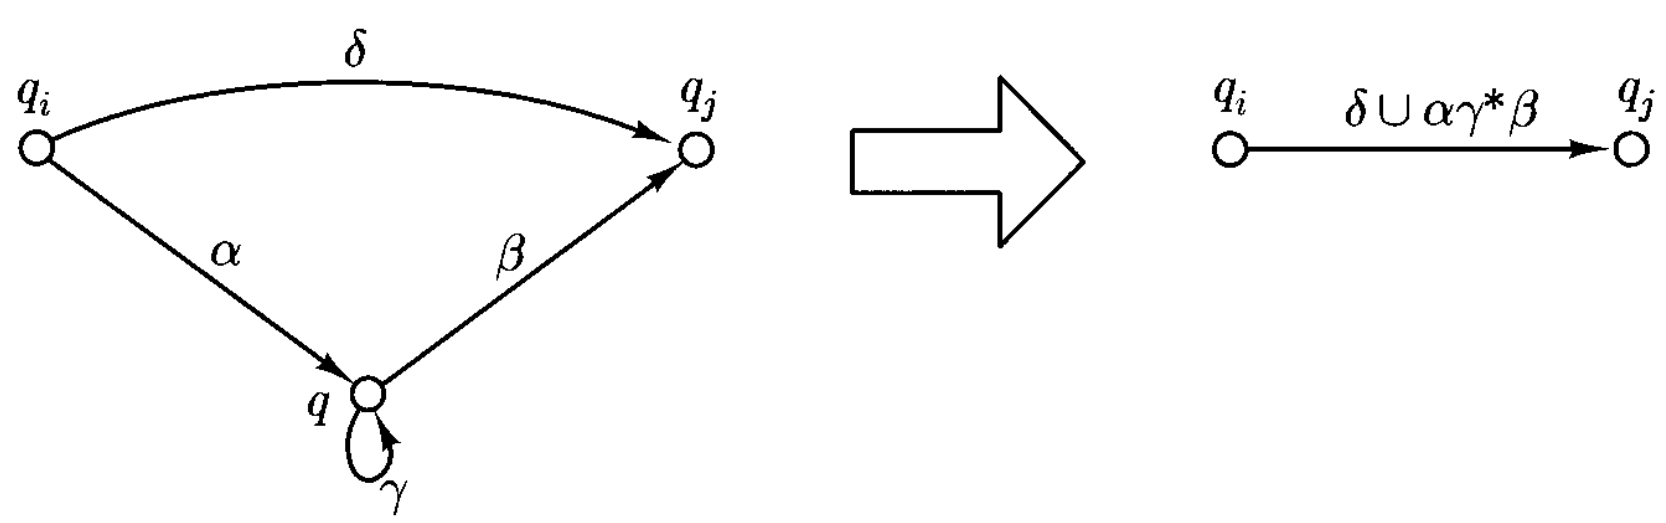
\includegraphics[width=.42\textwidth]{img/Fig2.17.png}
  \caption{}
\end{figure}
